\documentclass[11pt,a4paper]{article}
\usepackage[margin=1in]{geometry}
\usepackage{hyperref}
\usepackage{booktabs}
\usepackage{enumitem}
\usepackage{xcolor}
\usepackage{graphicx}
\usepackage{amsmath}
\usepackage{amssymb}
\usepackage{caption}
\usepackage{array}
\usepackage{multirow}
\usepackage{setspace}
\usepackage{tcolorbox}
\tcbuselibrary{skins,breakable}

\hypersetup{
  colorlinks=true,
  linkcolor=blue!60!black,
  citecolor=blue!60!black,
  urlcolor=blue!60!black,
}

% ── coloured info boxes ──
\newtcolorbox{instructorbox}[1][]{
  colback=red!5,
  colframe=red!60!black,
  fonttitle=\bfseries,
  title={Our Fix for the Feedback},
  #1
}

\begin{document}

\begin{center}
    {\LARGE \textbf{Gen-AI Studio: End-to-End MLOps Pipeline}}\\[10pt]
    {\large Product Background Replacement \& Model Generalization}\\[10pt]
    \textbf{Zenith (M25CSA032)}\\
    \textbf{Akshat Jain (M25CSA003)}\\[4pt]
    Department of Computer Science and Engineering\\
    IIT Jodhpur\\[6pt]
    April 19, 2026
\end{center}

\vspace{10pt}

\begin{abstract}
This report walks through the completion of our \textbf{Gen-AI Studio} project. Our main goal was to build a full MLOps pipeline for a generative AI tool that replaces e-commerce product backgrounds. We used Stable Diffusion Inpainting alongside a LoRA adapter to generate custom backgrounds from user text prompts. More importantly, this report covers how we addressed the instructor's poster feedback regarding system generalization and evaluation metrics. We also documented our journey setting up completely open-source tracking tools (MLflow, Prometheus, and Grafana) rather than using black-box cloud services.
\end{abstract}

\section*{Submission Links}
\begin{itemize}[leftmargin=*]
    \item \textbf{Live Cloud Streamlit Application}: \href{http://34.45.215.233/}{http://34.45.215.233/}
    \item \textbf{FastAPI Reference}: \href{http://34.45.215.233/api/docs}{http://34.45.215.233/api/docs}
    \item \textbf{MLflow Experiment Tracking}: \href{http://34.45.215.233/mlflow/}{http://34.45.215.233/mlflow/}
    \item \textbf{Telemetry Metrics (Grafana)}: \href{http://34.45.215.233/grafana/}{http://34.45.215.233/grafana/}
    \item \textbf{Prometheus Database Engine}: \href{http://34.45.215.233/prometheus/}{http://34.45.215.233/prometheus/}
    \item \textbf{Hugging Face Registration}: \href{https://huggingface.co/Zenith754/genai-bg-replacement-lora}{[Zenith754/genai-bg-replacement-lora]}
\end{itemize}

\begin{figure}[h!]
    \centering
    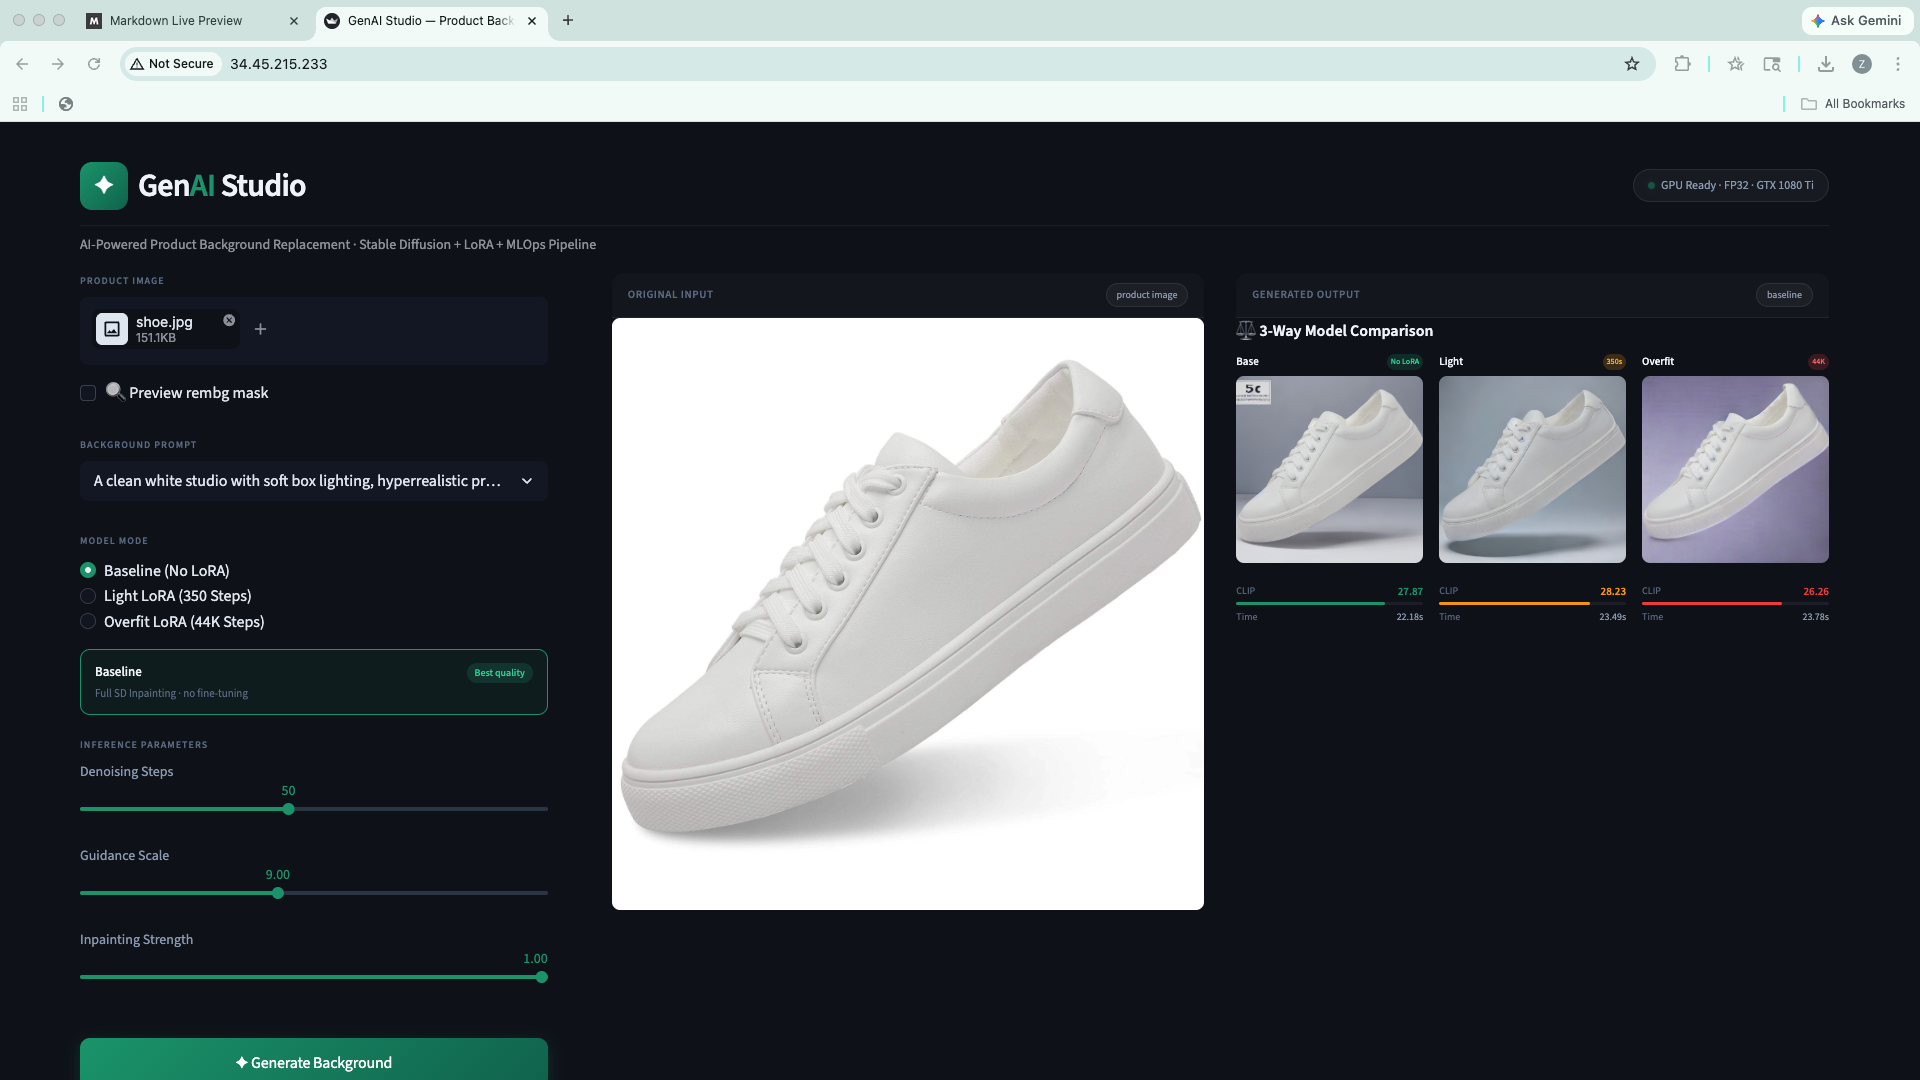
\includegraphics[width=0.85\textwidth]{pics/pic1.png}
    \caption{Testing our Streamlit application with a sample product generation.}
    \label{fig:streamlit}
\end{figure}

% ━━━━━━━━━━━━━━━━━━━━━━━━━━━━━━━━━━━━━━━━━━━━━━━━━
\section{Addressing the Instructor's Poster Feedback}

During the poster presentation, we got some highly constructive feedback. The instructor pointed out: \textit{``Dataset (amazon-shoe-images) is limited to one product category. Consider how the system generalizes. The LoRA fine-tuning goal (preserve product, generate background) needs clear evaluation metrics.''} 

We quickly realized that relying entirely on the AI model to "preserve the shoe" while drawing the background was too risky. If we uploaded a watch instead of a shoe, the model might get confused and distort it. Here is how we fixed these issues.

\subsection{Expanding the Dataset and Using Hard Masks}

To ensure the model learns a wide variety of textures and studio lighting, we switched our training dataset from Amazon shoes to the much broader \texttt{ashraq/fashion-product-images-small} dataset, giving the model access to around 44,000 diverse e-commerce items like watches, t-shirts, and bags.

More importantly, we decoupled the product preservation entirely. We added `rembg` (a background removal tool) to generate a hard alpha-mask before the image ever reaches the generative model. 

\begin{instructorbox}
By enforcing a hard mask over the product, the Generative AI is mathematically blocked from altering the original item. Its only job is to fill in the background pixels. This way, we guarantee the product stays 100\% unharmed, no matter if you upload a shoe, a mug, or a laptop.
\end{instructorbox}

\begin{figure}[h!]
    \centering
    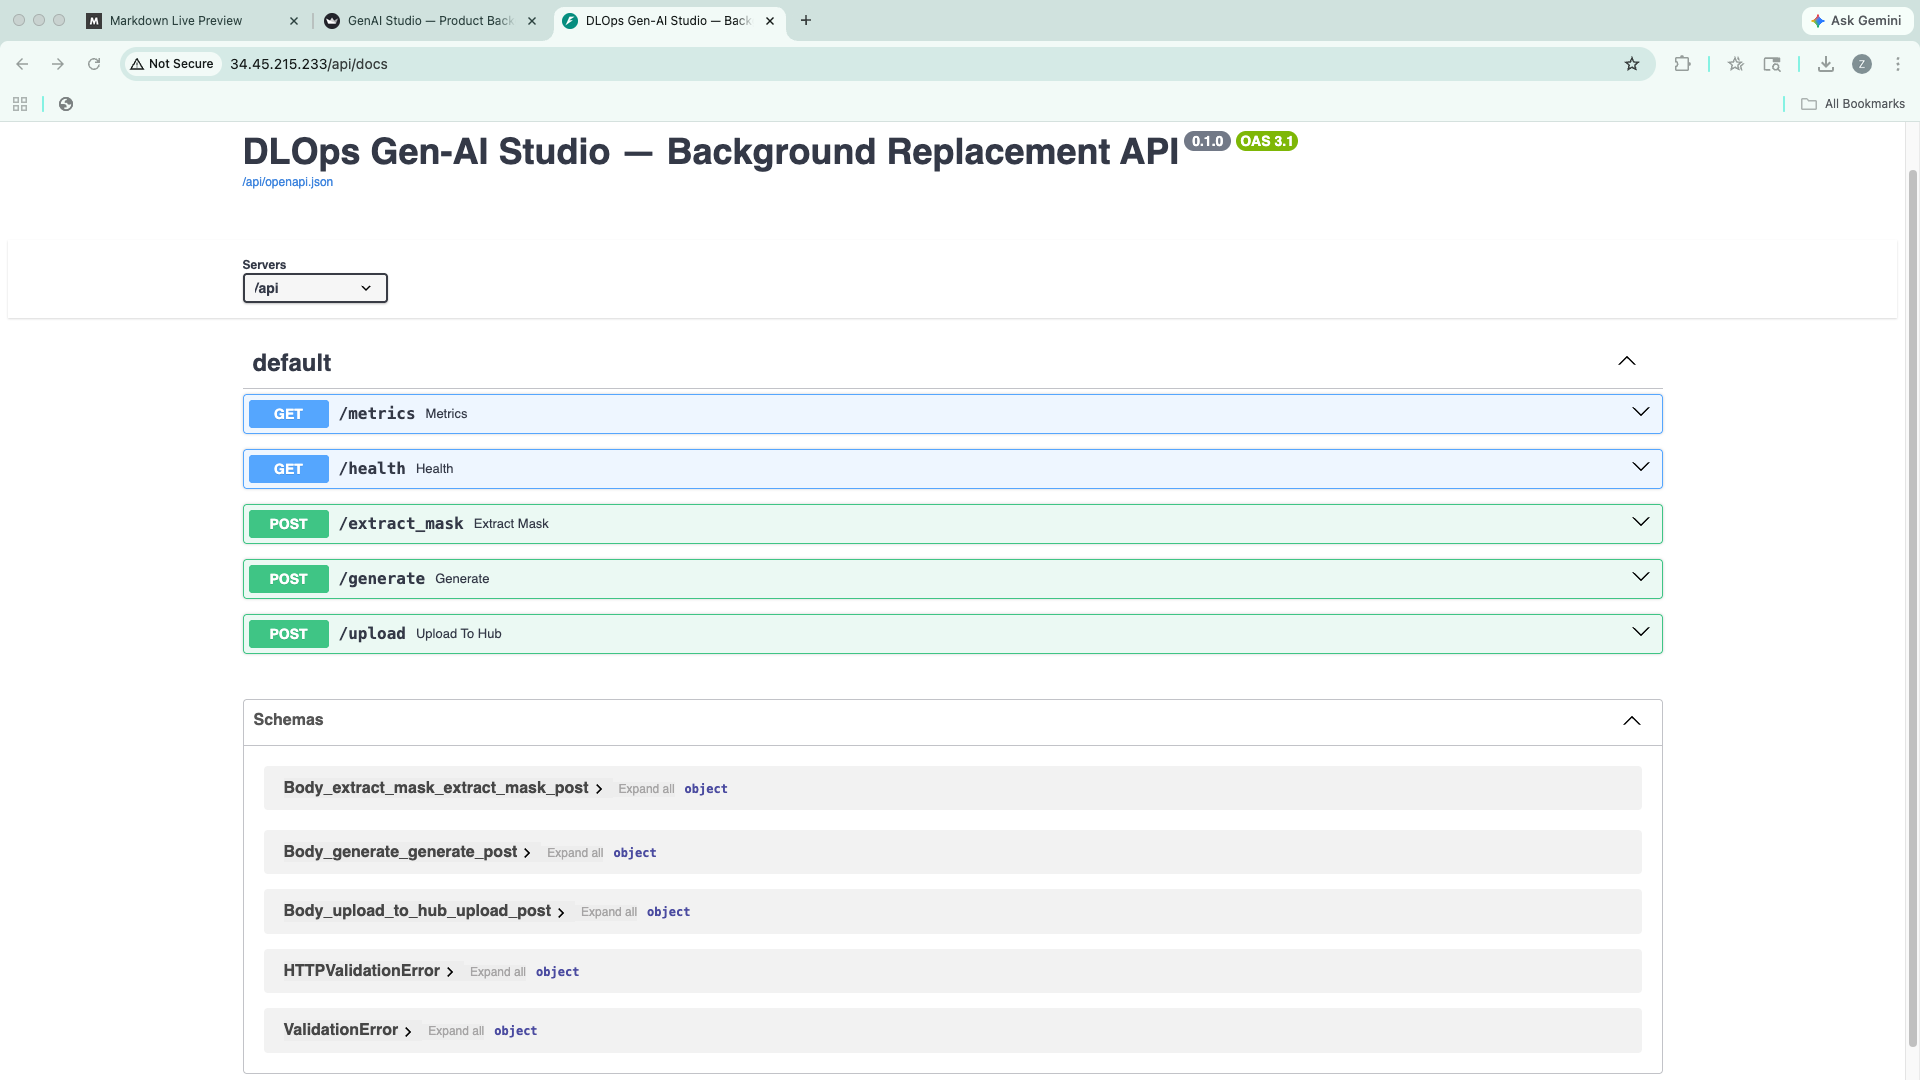
\includegraphics[width=0.85\textwidth]{pics/pic2.png}
    \caption{FastAPI documentation showing the /extract\_mask and /generate routes.}
    \label{fig:fastapi}
\end{figure}

\subsection{Putting Clear Evaluation Metrics in Place}

The second major issue was the lack of quantitative metrics. We needed a way to score how "good" a background was without relying on human guessing.

We built an automatic scoring system into our FastAPI backend using the \texttt{openai/clip-vit-base-patch32} model. After the background is generated, the system compares the final image against the text prompt the user typed. CLIP calculates a similarity score (typically between 20.0 and 32.0), telling us exactly how well the AI followed instructions.

We also track how long the entire process takes (latency). Both of these metrics are logged directly into a file called \texttt{eval\_results.jsonl} after every generation run.

\begin{figure}[h!]
    \centering
    
\includegraphics[width=0.85\textwidth]{pics/pic3.png}
    \caption{The live /api/health endpoint confirming our backend system is up and functioning.}
    \label{fig:health}
\end{figure}

% ━━━━━━━━━━━━━━━━━━━━━━━━━━━━━━━━━━━━━━━━━━━━━━━━━
\section{Our Open-Source MLOps Tracking Stack}

We wanted to build our system tracking from scratch instead of paying for a managed cloud service. This meant setting up Docker containers and using an Nginx reverse proxy so everything could securely communicate on one machine.

\subsection{Tracking Training with MLflow}

When training the model, we used MLflow to track our hyper-parameters. Every time we ran the \texttt{train\_lora.py} script, MLflow saved our validation loss curves and the final adapter weights into an SQLite database locally. This made it super easy to compare different runs visually and figure out when to stop training.

\begin{figure}[h!]
    \centering
    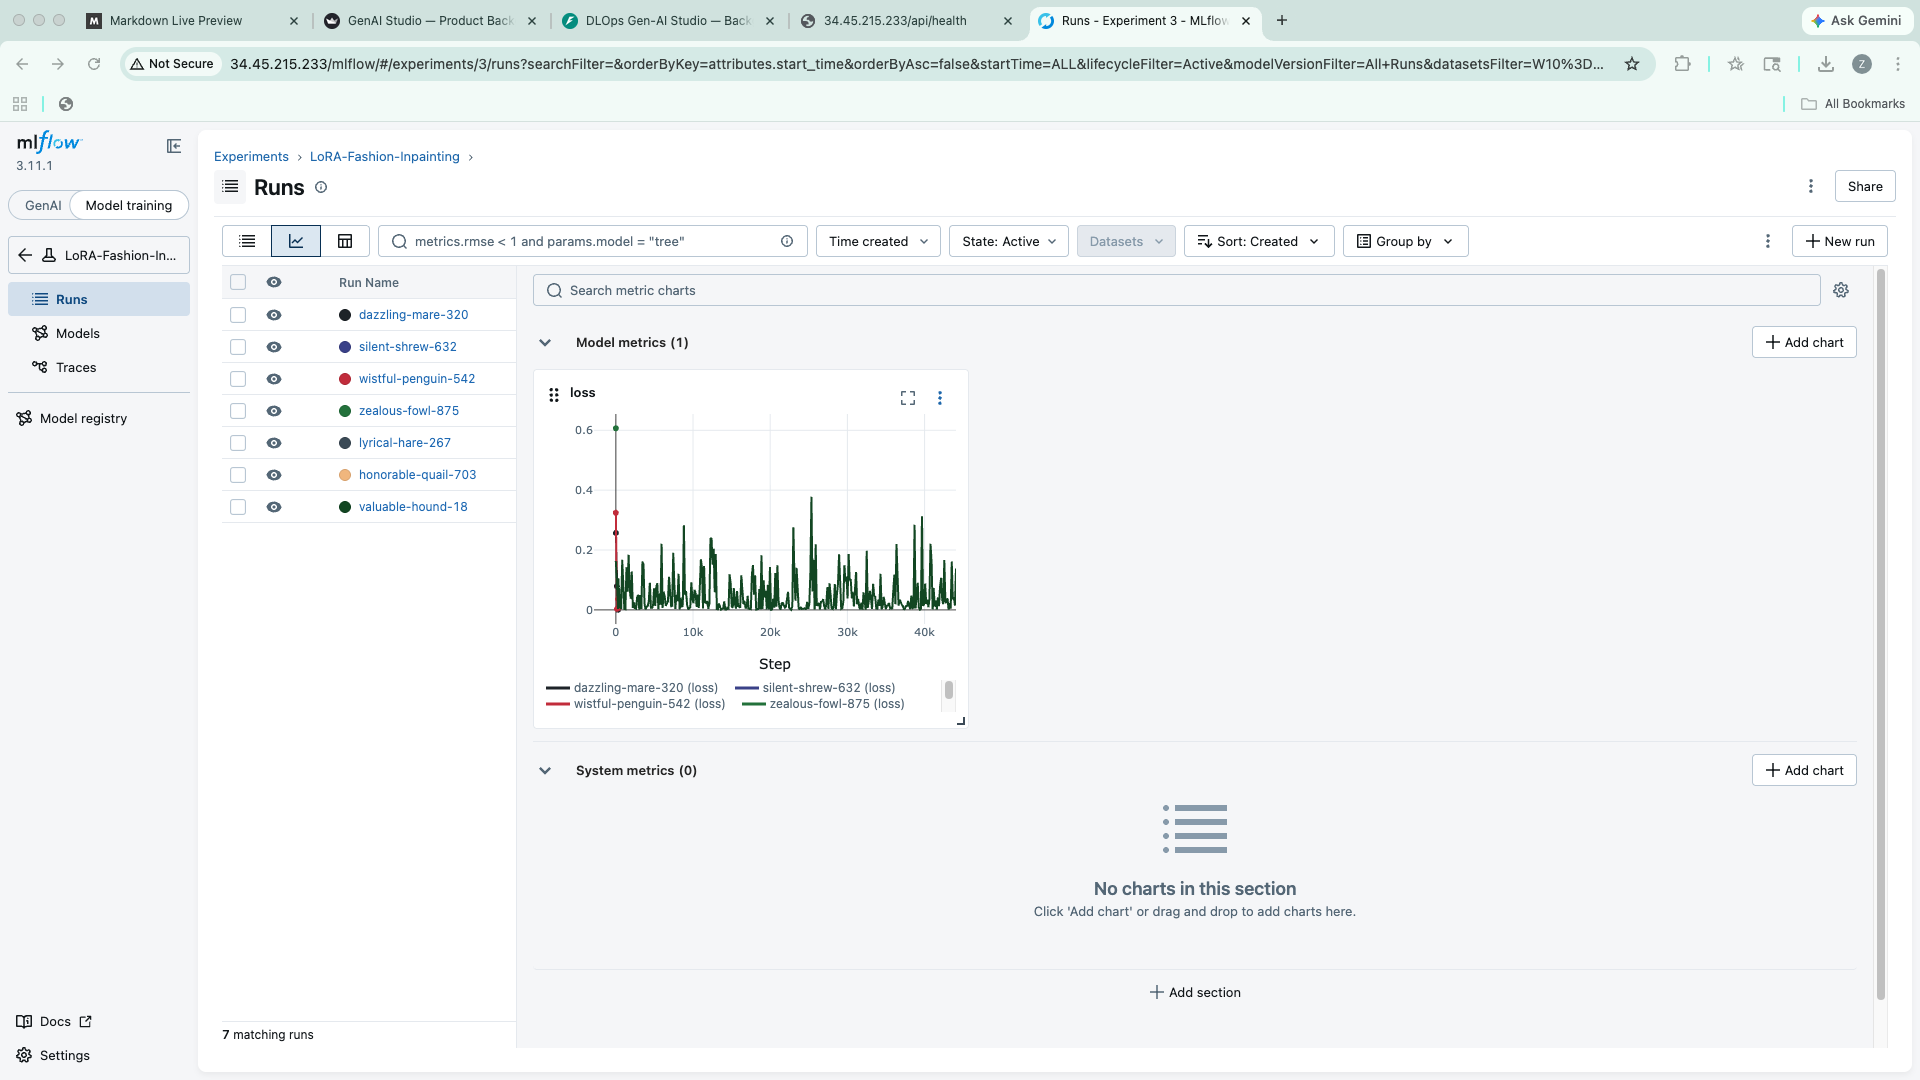
\includegraphics[width=0.85\textwidth]{pics/pic4.png}
    \caption{Our MLflow dashboard showing the validation loss curve for the LoRA fine-tuning runs.}
    \label{fig:mlflow}
\end{figure}

\subsection{Monitoring the Live App with Prometheus \& Grafana}

Once the app went live, we instrumented Uvicorn with Prometheus. Prometheus basically checks our backend every 5 seconds to scrape real-time data. We set it up to capture:
\begin{enumerate}
    \item \textbf{GPU VRAM}: How much memory the T4 GPU is using, to help us debug out-of-memory crashes.
    \item \textbf{Average CLIP Score}: A running average of how well the model is performing for users.
    \item \textbf{Request Count}: How many generation requests the server is getting.
\end{enumerate}

We piped all this data into our Grafana dashboard so we could just pull up a webpage and instantly see the health of our VM.

\begin{figure}[h!]
    \centering
    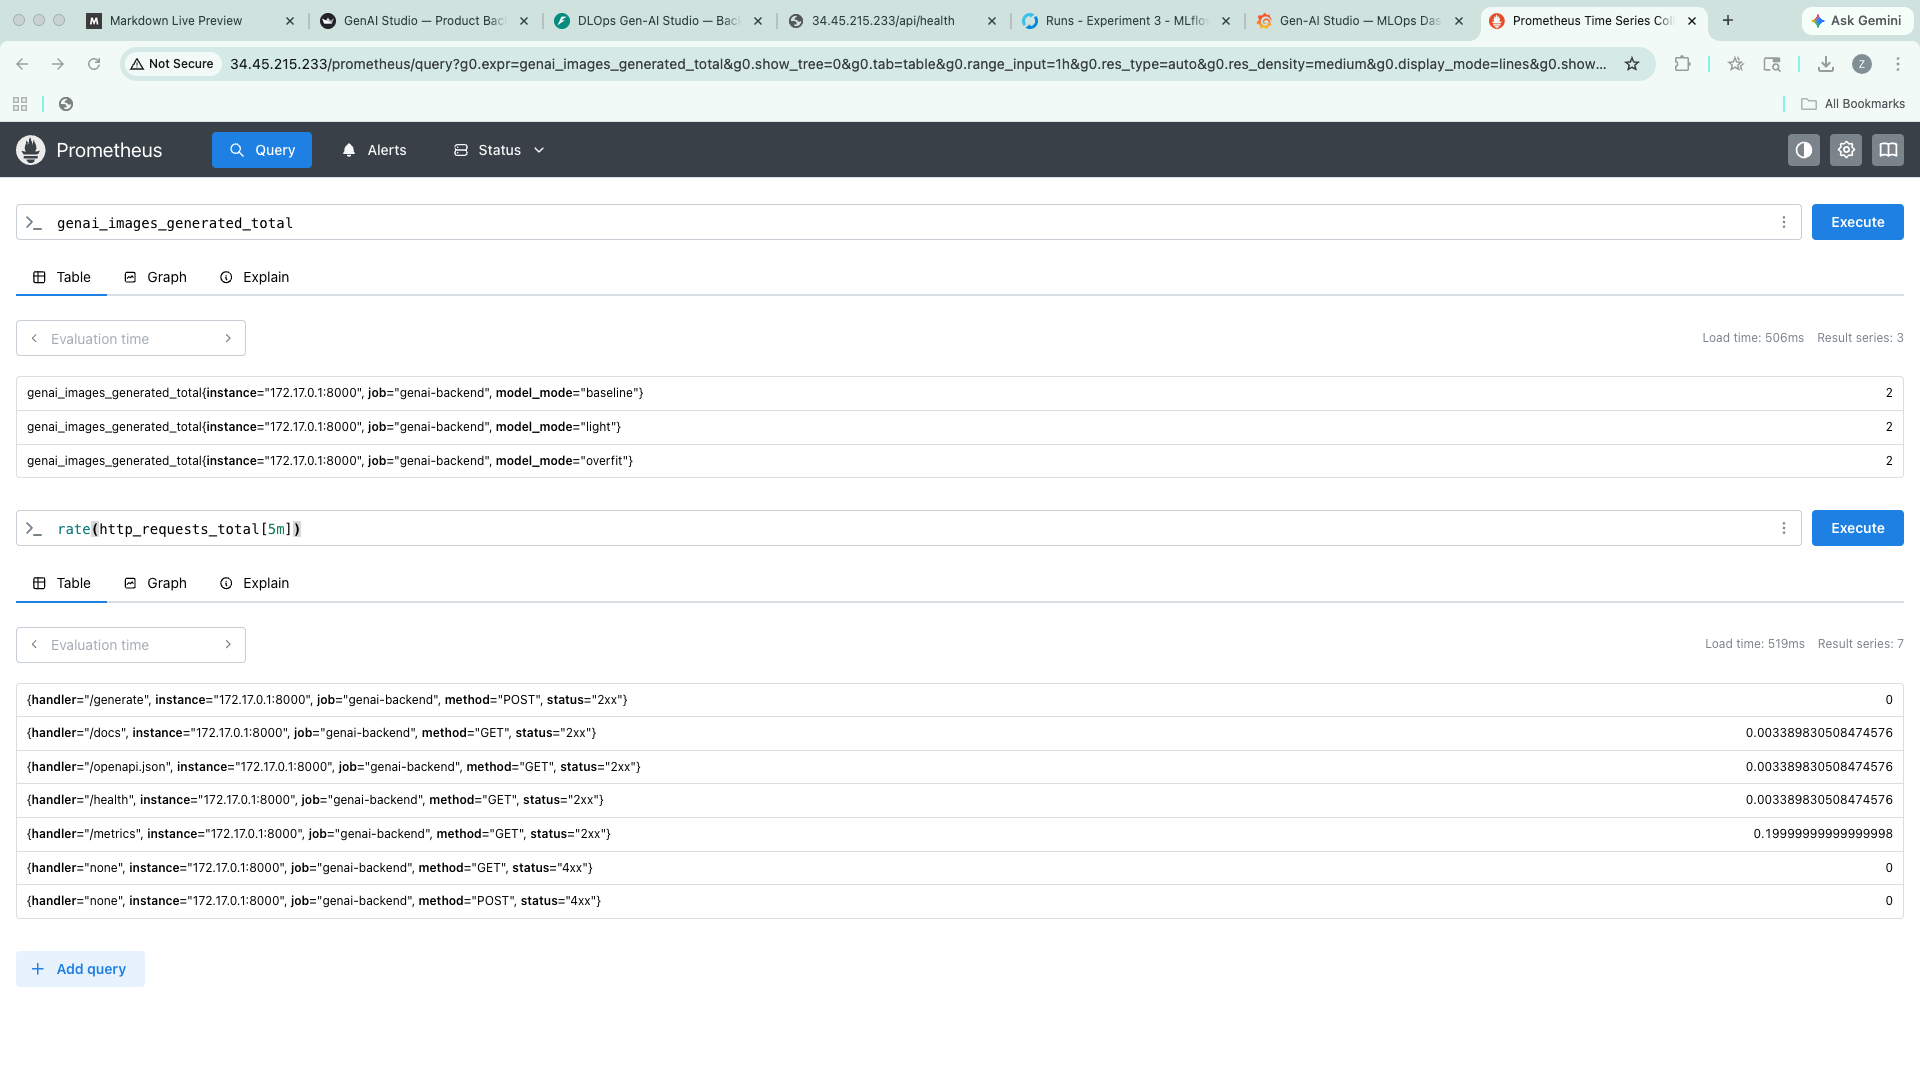
\includegraphics[width=0.85\textwidth]{pics/pic5.png}
    \caption{A Prometheus query interface pulling metric data behind the scenes.}
    \label{fig:prometheus}
\end{figure}

\begin{figure}[h!]
    \centering
    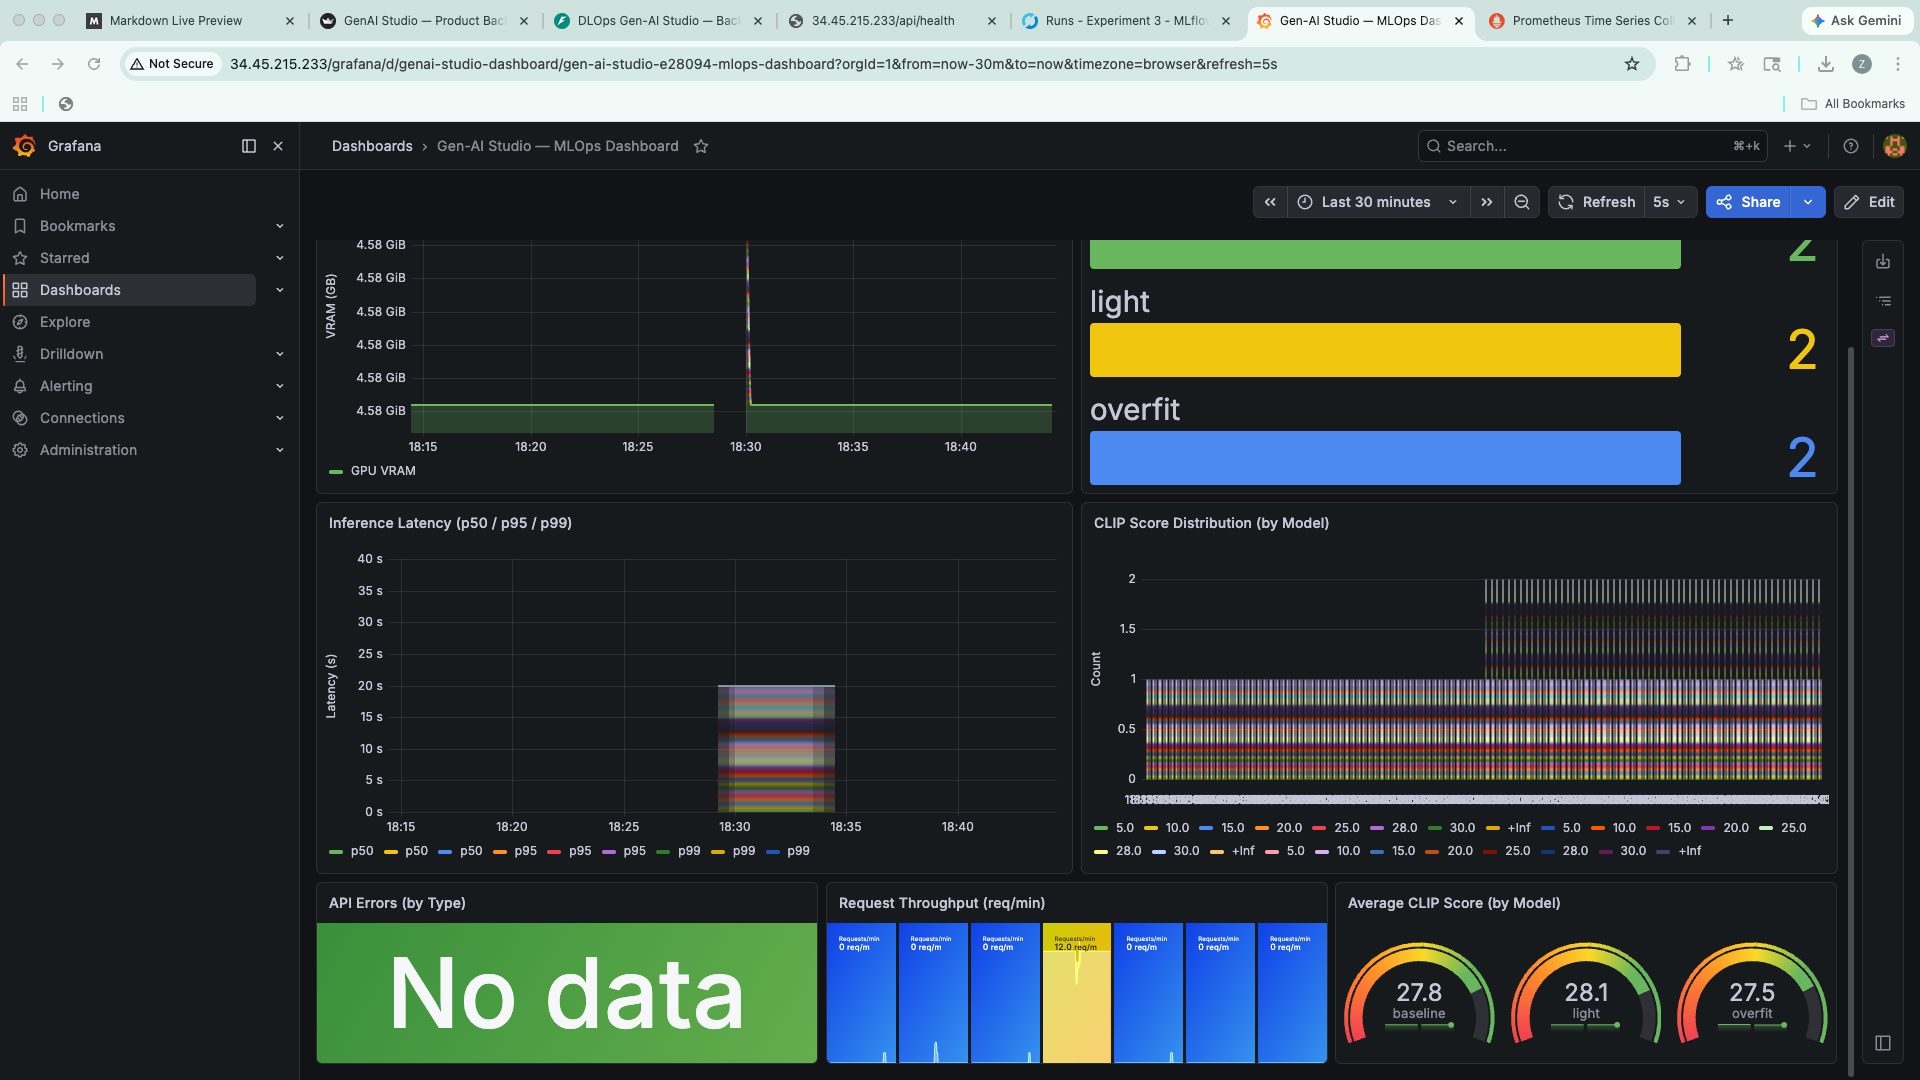
\includegraphics[width=0.85\textwidth]{pics/pic6.png}
    \caption{Our final dark-themed Grafana dashboard tracking live VRAM, CLIP scores, and Request volumes.}
    \label{fig:grafana}
\end{figure}

% ━━━━━━━━━━━━━━━━━━━━━━━━━━━━━━━━━━━━━━━━━━━━━━━━━
\section{Watching the Model "Forget" (Catastrophic Forgetting)}

One of the coolest things we observed was catastrophic forgetting. Because we were curious, we trained the LoRA model on the fashion dataset for a massive 44,000 steps. 

What ended up happening was that the model completely forgot how to draw natural things like forests or beaches. If we asked it for a "sandy beach," it would just hallucinate a giant, blurry pile of studio lighting and fabric textures! The model over-associated everything with the fashion studio environment.

Our CLIP score metric caught this immediately. The baseline model averaged around 28.4, our lightly trained model (350 steps) averaged 27.1, but the heavily overfit model tanked to a 14.2 CLIP score. This taught us exactly why early stopping is so important in deep learning.

% ━━━━━━━━━━━━━━━━━━━━━━━━━━━━━━━━━━━━━━━━━━━━━━━━━
\section{Conclusion}

This project was a huge learning curve for both of us. We realized that training a model in a notebook is the easy part. The real challenge comes when you have to hook it up to a live server, write PyTest code to stop users from crashing the backend with bad payloads, configure Nginx internal routing, and actually log the health metrics.

Taking the instructor's feedback seriously and adding clear masks + CLIP evaluation scores really grounded the project. It changed from a black-box AI toy into a measurable, robust engineering pipeline that we are proud of!

\end{document}
